\documentclass{article}

\usepackage{hyperref}

% Below will configure hyperlink colors
\hypersetup{
    colorlinks=true,
    linkcolor=blue,
    filecolor=blue,
    urlcolor=blue,
}
\urlstyle{same}

\usepackage{enumitem}

% Below package is for precise positioning of images
\usepackage{float}
\usepackage{color}

% Below package is for syntax highlighted code
\usepackage{minted}
% Below set global setting fro minted package like line wraps and frame
\setminted{breaklines, frame=single}

% Below package is for including images
\usepackage{graphicx}
\usepackage[a4paper, inner=1.5cm, outer=3cm, top=2cm,bottom=3cm, bindingoffset=1cm]{geometry}
\setlength{\parskip}{.5em}

% The LaTeX graphics/graphicx package uses the first dot to find the extension. Package grffile changes this algorithm. This helps in including images files whose name contains more than 1 dot
\usepackage{grffile}


% Below package will create headings
%\pagestyle{headings}

% Below package will used to specify captions like "Figure 1: Nice Figure" in minipages using \captionof{figure}{Nice Figure}
\usepackage{caption}
\usepackage{hypcap} %This is needed for some warning in minipages


\begin{document}
\begin{titlepage}
   \vspace*{\stretch{1.0}}
   \begin{center}
      \Large\textsc{Setting user mode break points from KD aka .process /i vs .process /r /p}\\
      \vspace{5mm}
      \Large\textit{Vineel Kovvuri}\\
      \url{http://vineelkovvuri.com}\\
   \end{center}
   \vspace*{\stretch{2.0}}
\end{titlepage}

\tableofcontents

\newpage
\section{Introduction}
When performing KD(Kernel Debugging) in Windows with Windbg if you have to set a break point in a user mode process we should always use .process /i address; g; .reload /user. Lot of good content is written on the internet on this command, but nothing seemed to explain why this command should be used instead of the familiar .process /r /p address. I would like to shed some light on this. Before reading any further I would strongly encourage you to read about it from above link. In this article I assume some basic knowledge on how kernel debugging is done with Windbg. Also, I would like to start with the following question.

\textit{If the debugger has read/write access to the user mode process via .process /r /p why cannot it insert int 3 in user mode process when performing KD? Why do we have to make the user mode process the current process context by running .process /i ?}

To explain this we need to quickly understand how break points work.


\section{How do break points work in user mode debugging}
How do break points work in user mode debugging
Below are the steps involved for a break point to work in debugging a user mode process.

\begin{enumerate}[noitemsep]
    \item bp address – you are just instructing the debugger to make a note of “address” and replace the byte at that address with 0xcc (int 3) when target resumes to execute
    \item g – when you hit “g” the debugger replaces the byte with 0xcc and stores the original byte with it
    \item After execution when processor execute the modified byte (0xcc) this causes the debugger to break in and debugger puts back the original byte as if nothing has happened to the program
    \item More details: \url{http://vineelkovvuri.com/2016/09/04/how-does-breakpoints-work-in-debuggers/}
\end{enumerate}


\section{User mode break points from KD}
When debugging a user mode process from KD the steps works exactly same as above but with a slight twist.
\begin{enumerate}[noitemsep]
    \item Let’s assume during KD, when the debugger broke, the processor is executing a process named mulithasher.exe(see note below)
    \item When you switch the windbg’s view to a different process(fscapture.exe) by .process /r /p <fscapture address>, you are not changing the underlying execution of the processor. !process -1 0 still shows multihasher.exe
    \begin{enumerate}[noitemsep]
    \item With /r /p you now have read/write access to the fscapture process. This confirms the first part of the question
    \end{enumerate}
    \item bp address  – same as above, you are instructing the debugger to make a note of “address” and replace the byte at that address with 0xcc (int 3) when target resumes to execute
    \item when you hit “g” the debugger replaces the byte at address with 0xcc in the currently executing process which happens to be multihasher.exe not fscapture.exe!

    \item
    \begin{minipage}{\linewidth}
    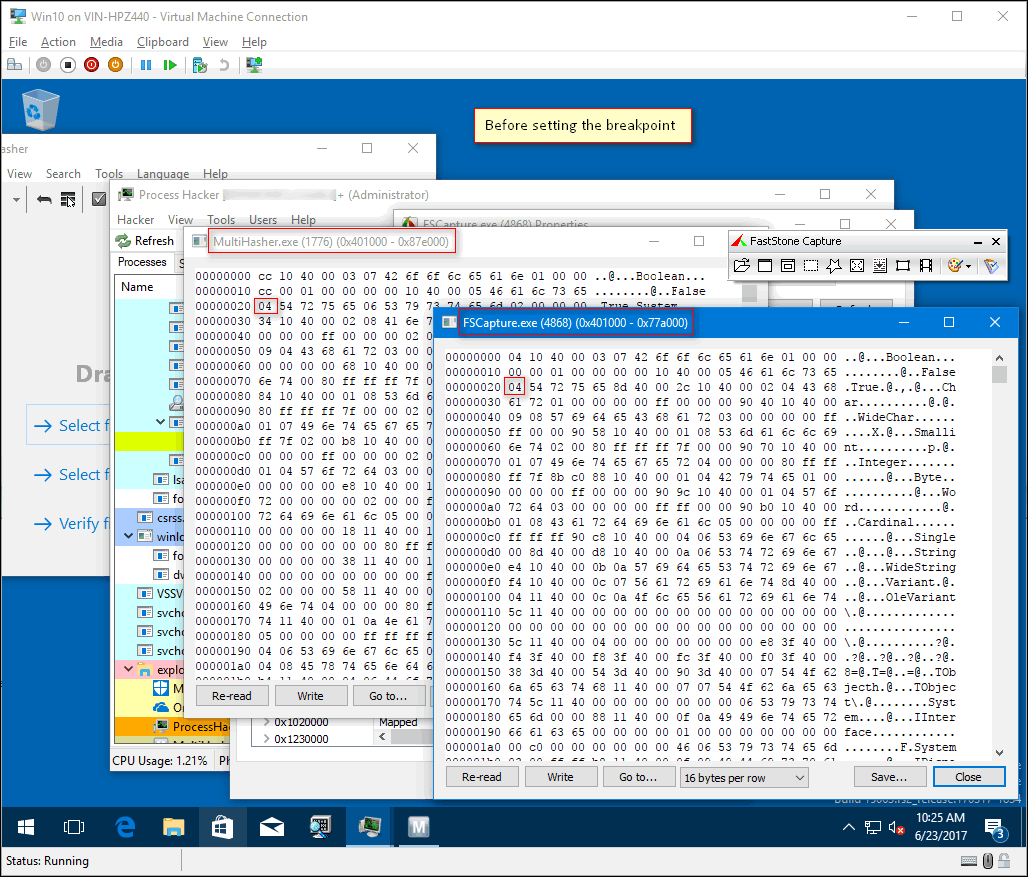
\includegraphics[width=\linewidth]{UsermodeBreakPointFromKD1.png}
    \captionof{figure}{Before break point getting updated }
    \end{minipage}

    \item
    \begin{minipage}{\linewidth}
    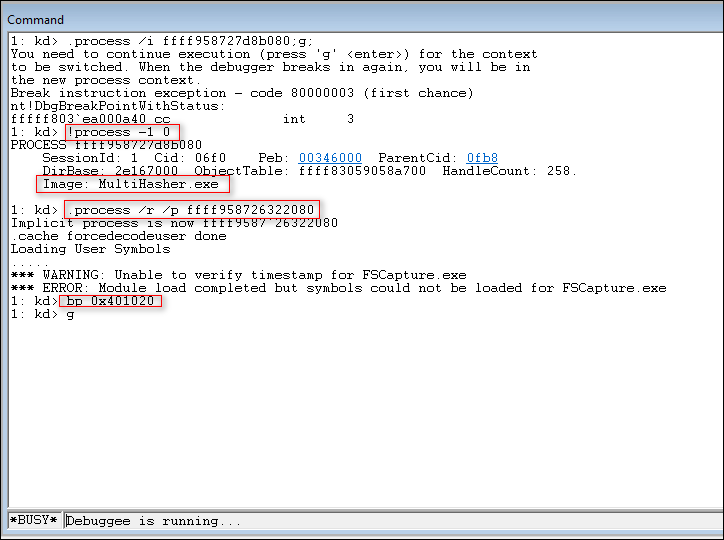
\includegraphics[width=\linewidth]{UsermodeBreakPointFromKD2.png}
    \captionof{figure}{Setting the break point  }
    \end{minipage}

    \item
    \begin{minipage}{\linewidth}
    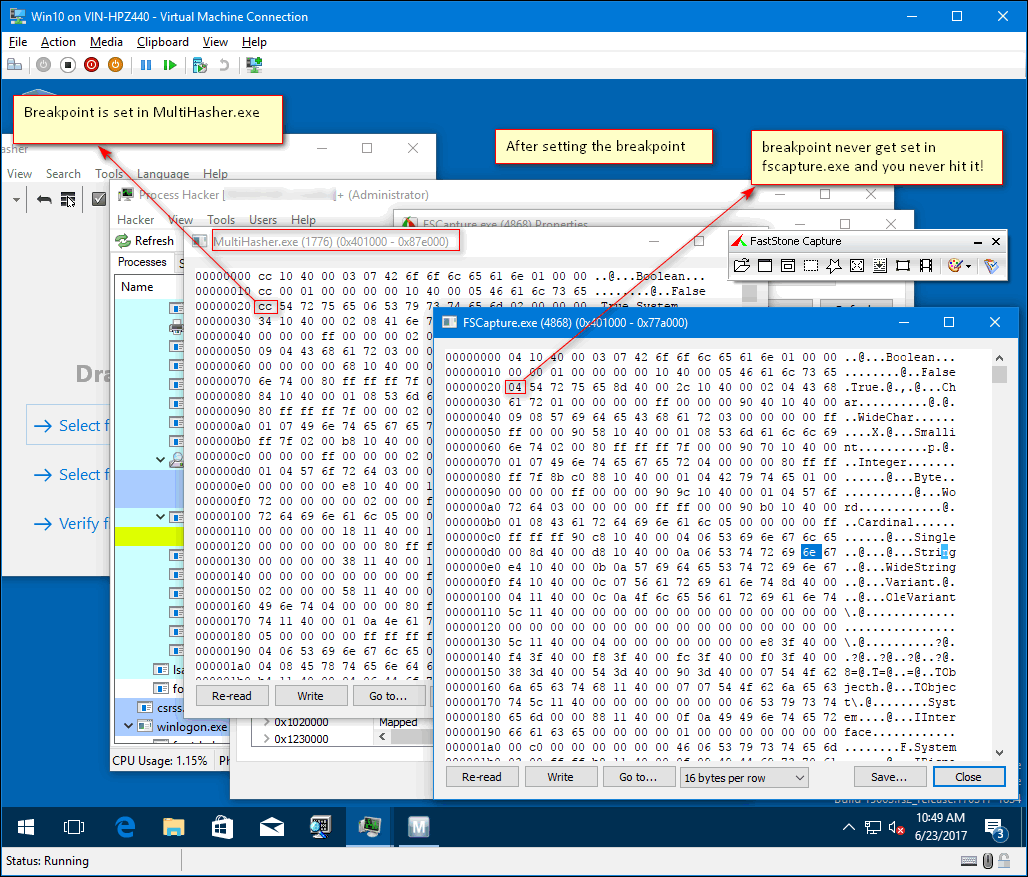
\includegraphics[width=\linewidth]{UsermodeBreakPointFromKD3.png}
    \captionof{figure}{After break point is updated }
    \end{minipage}

    \item This means, “g” command used to resume the target is the culprit(may be it is by design). This answers the second part of the question
    \item So by using .process /i <address>;g; windbg will break under your process context(how?). After which setting a break point and hitting “g” will cause the debugger to actually put int 3 in your process not somewhere else
\end{enumerate}
NOTE: I initially made multihasher.exe the process context by using .process /i <multihasher address>;g;
\section{Setting breakpoints in system dlls}
This .process /i is not required if you are putting breakpoints in system dlls like kernelbase, ntdll etc because these dlls are loaded at the same virtual address in all the user mode processes and they have a single copy in the physical memory. So once a break point set in a process the break point is visible in all other processes which uses that system dll. Below we illustrate this by setting a break point in ntdll.dll. (Even here just make sure when you broke initially you are not in System process as it will not have ntdll!)
\begin{enumerate}[noitemsep]
    \item
    \begin{minipage}{\linewidth}
    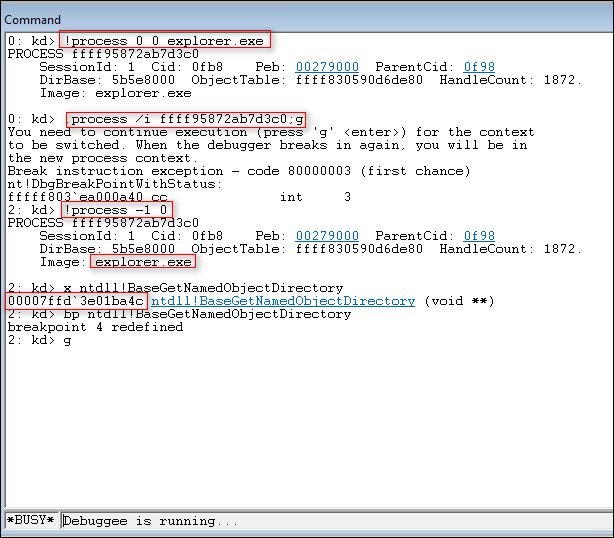
\includegraphics[width=\linewidth]{UsermodeBreakPointFromKD4.png}
    \captionof{figure}{Break point is set only in ntdll of explorer process}
    \end{minipage}

    \item
    \begin{minipage}{\linewidth}
    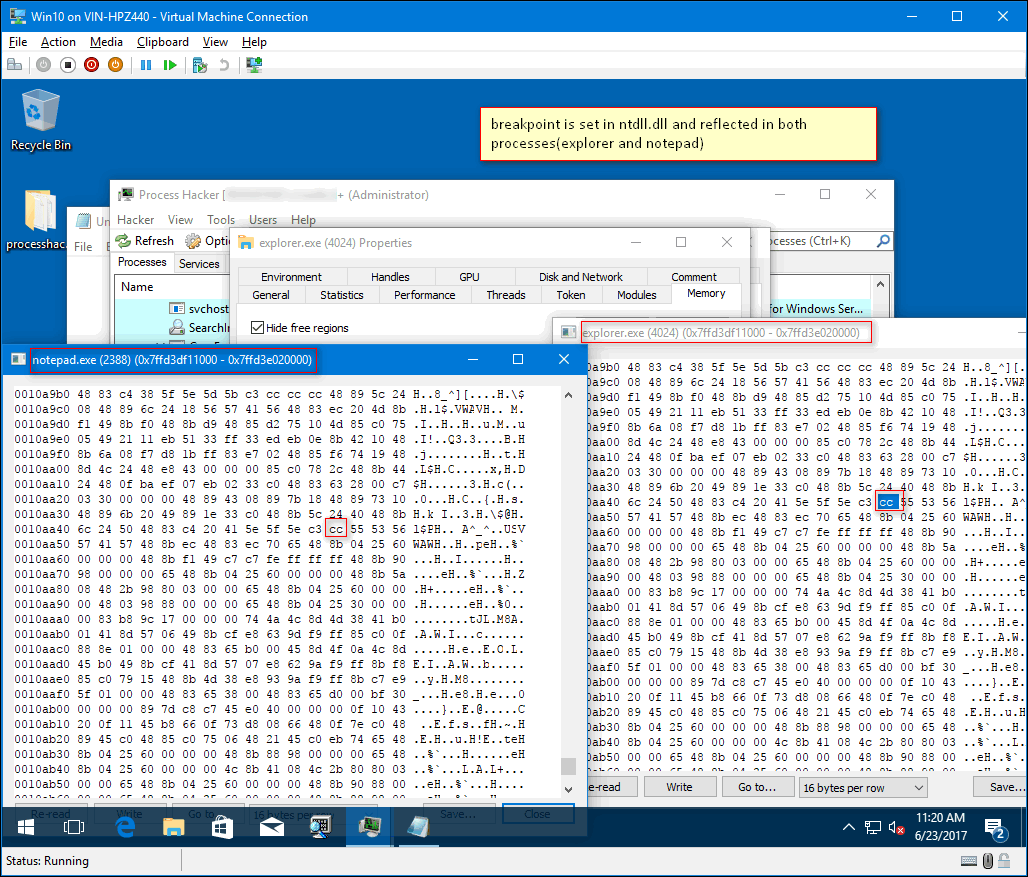
\includegraphics[width=\linewidth]{UsermodeBreakPointFromKD5.png}
    \captionof{figure}{Break point set in ntdll of explorer gets reflected in ntdll of notepad also}
    \end{minipage}
\end{enumerate}
\section{References}
\begin{enumerate}[noitemsep]
\item \href{http://www.osronline.com/article.cfm?id=576}{Analyst's Perspective: Analyzing User Mode State from a Kernel Connection}
\item \href{https://www.microsoftpressstore.com/articles/article.aspx?p=2201303&seqNum=2}{How Windows Debuggers Work?}
\end{enumerate}

\end{document}
